\begin{figure}[!hbt]
    \centering
    \begin{minipage}{0.45\textwidth}
        \centering
        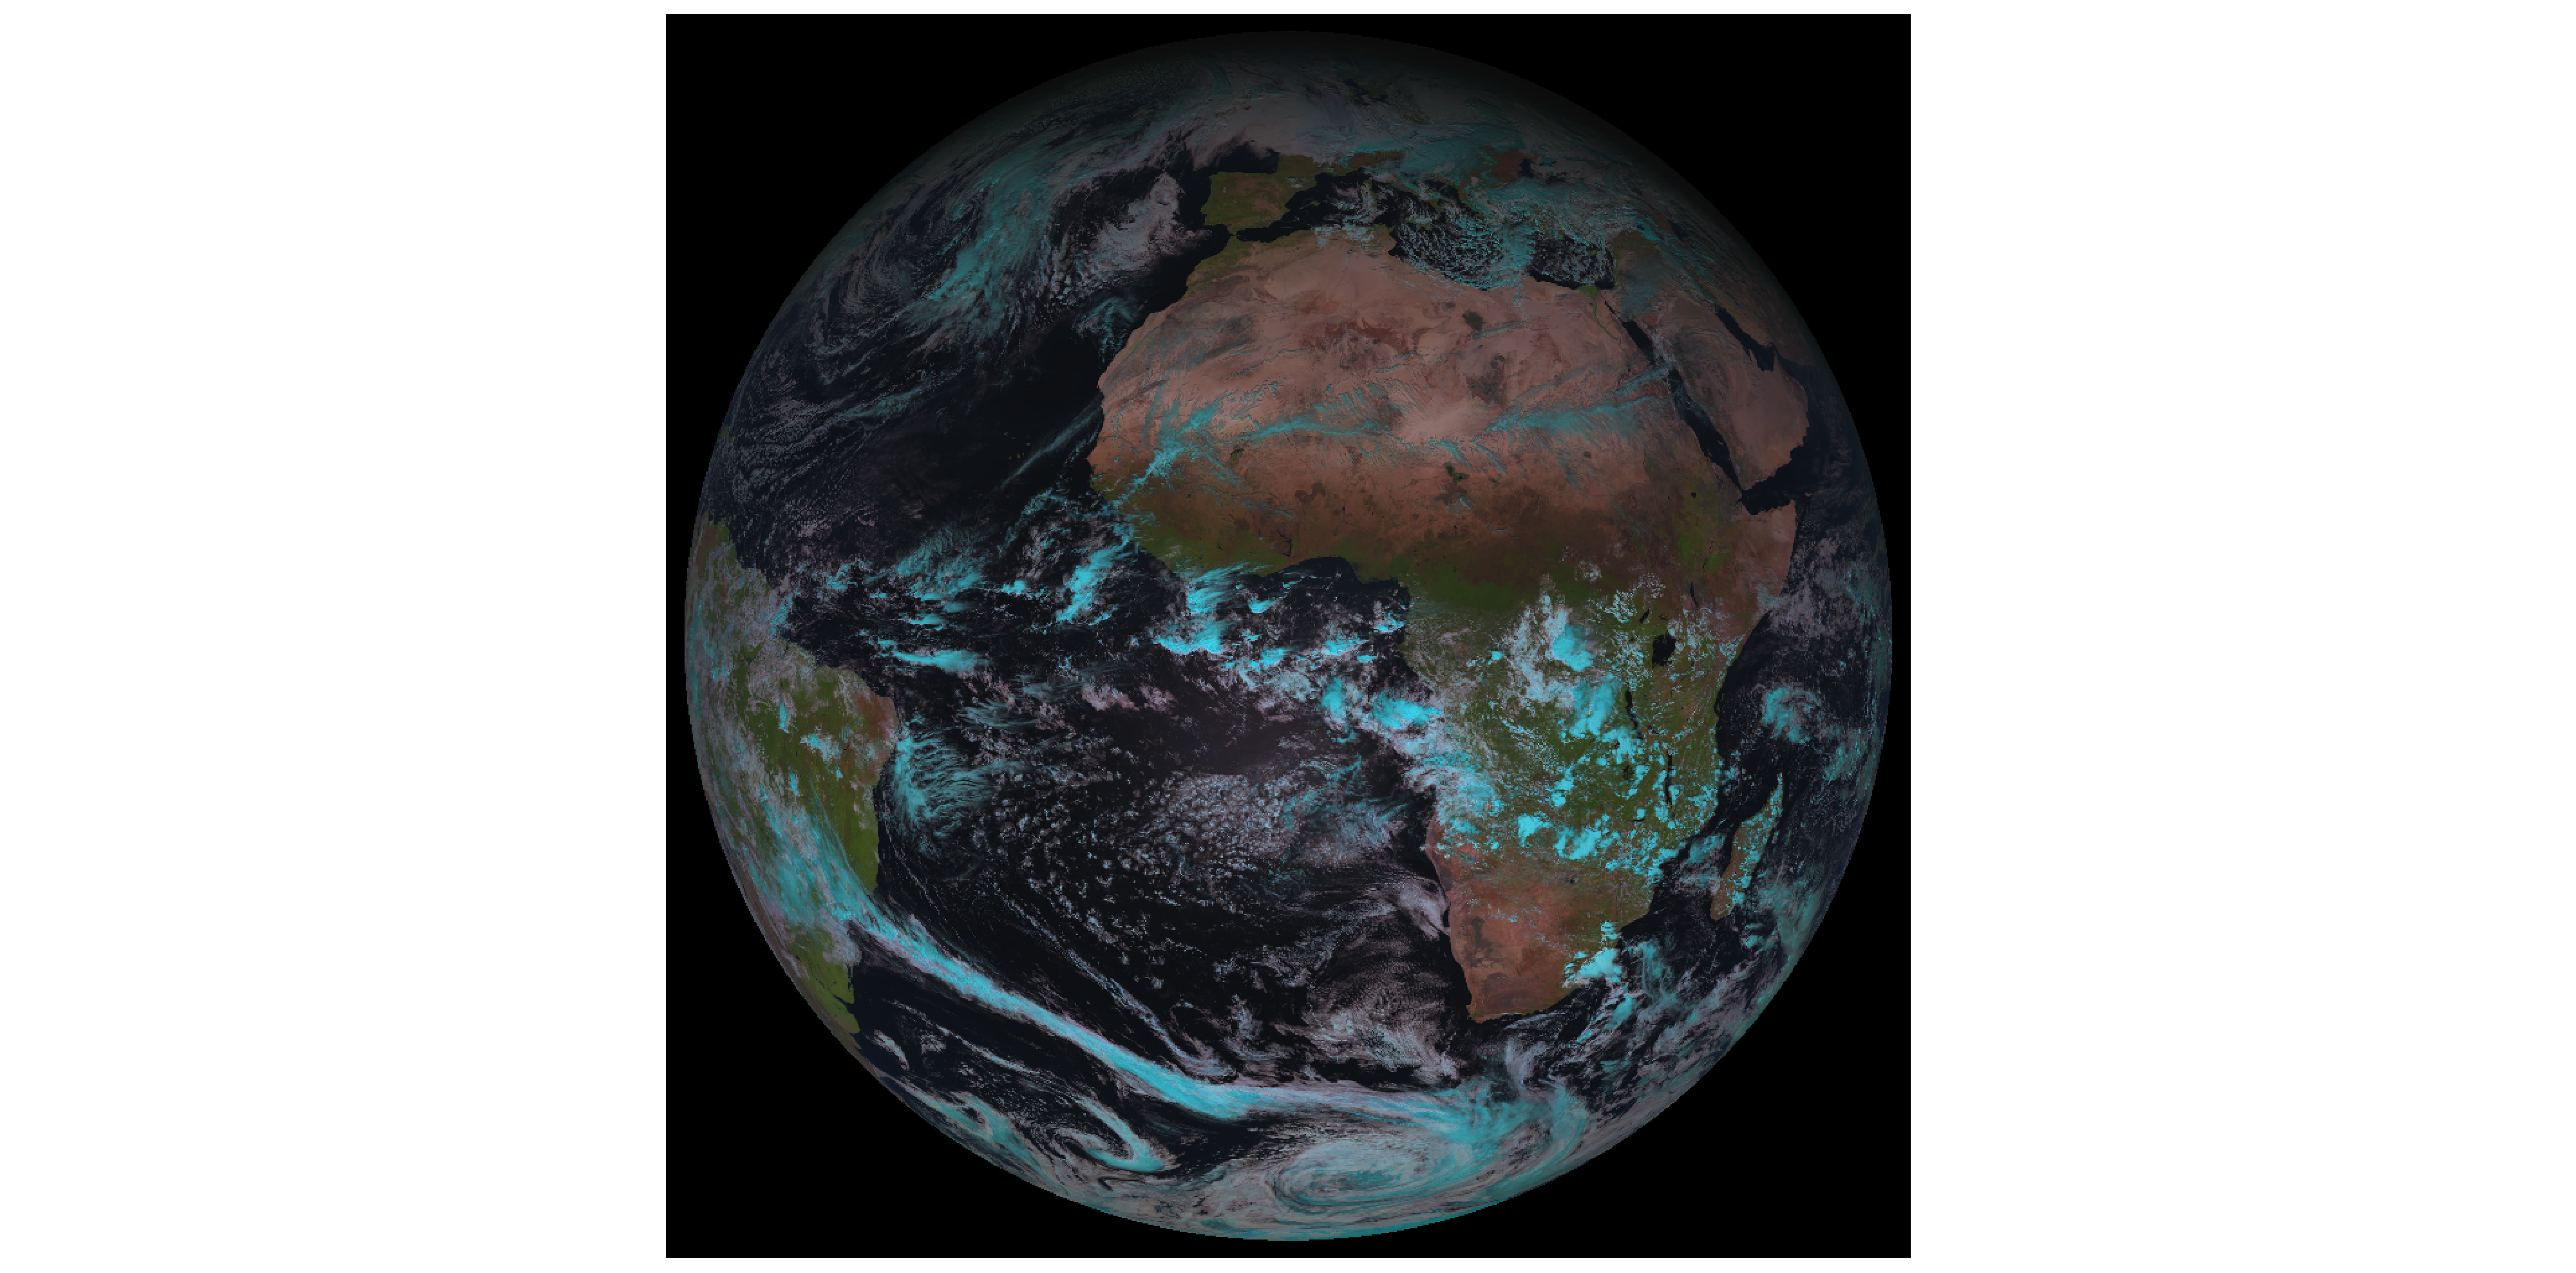
\includegraphics[width=0.9\textwidth]{2019-01-05 122743.pdf}
        \caption{RGB created from the stacking of the IR 1.6, VIS 0.6 and VIS 0.8 channel images for 2019-01-05 12:27:43 }
        \label{fig:av_rgb}
    \end{minipage}\hfill
        \begin{minipage}{0.45\textwidth}
        \centering
        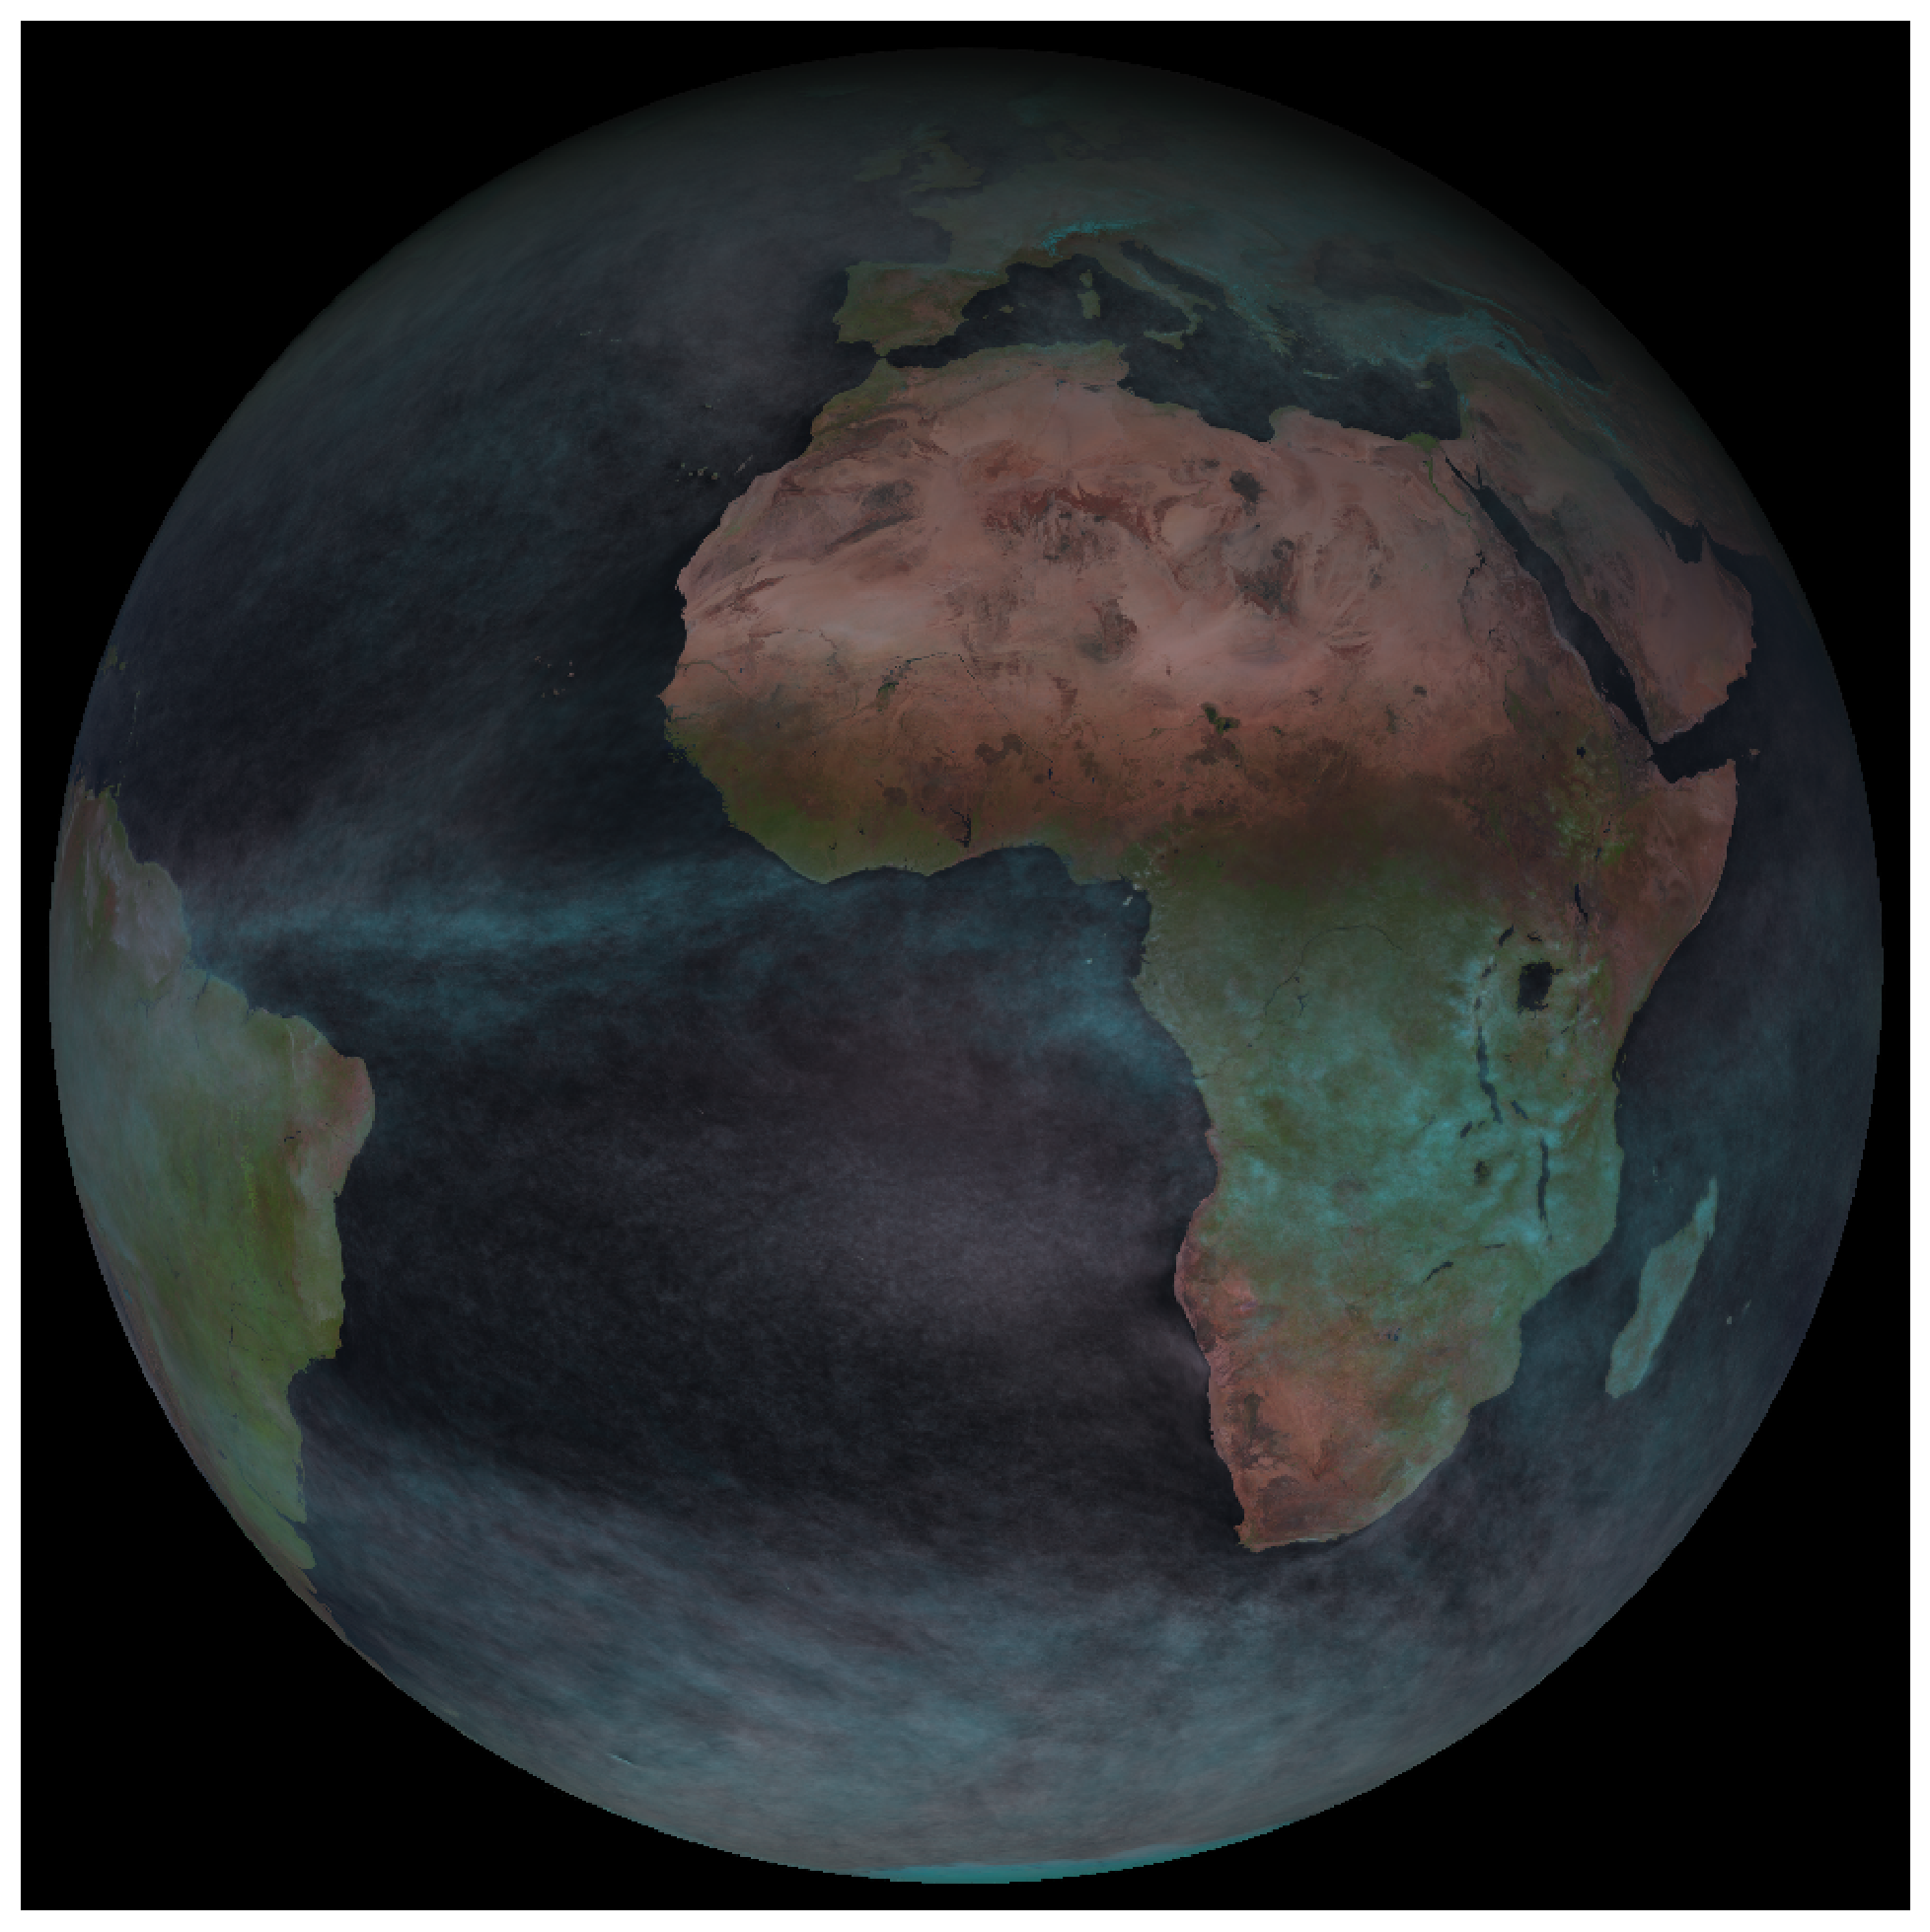
\includegraphics[width=0.9\textwidth]{2019-01-05 122743_av.pdf}
        \caption{RGB image formed from the averaging of all pixel values across the month of January 2019}
        \label{fig:av_cloud}
    \end{minipage}\hfill
\end{figure}

Fig.~\ref{fig:av_rgb} and Fig.~\ref{fig:av_cloud} both show an RGB colour image of the Earth in January 2019, created from data taken from Meteosat 9. The former consists of an RGB image, plotted using the channel data obtained at 12:27:43 on the 5th Janury 2019, while the latter was created through the addition and subsequent division of the corresponding pixel values across all the images taken in the month of January 2019. 

\begin{figure}[h]
    \centering
    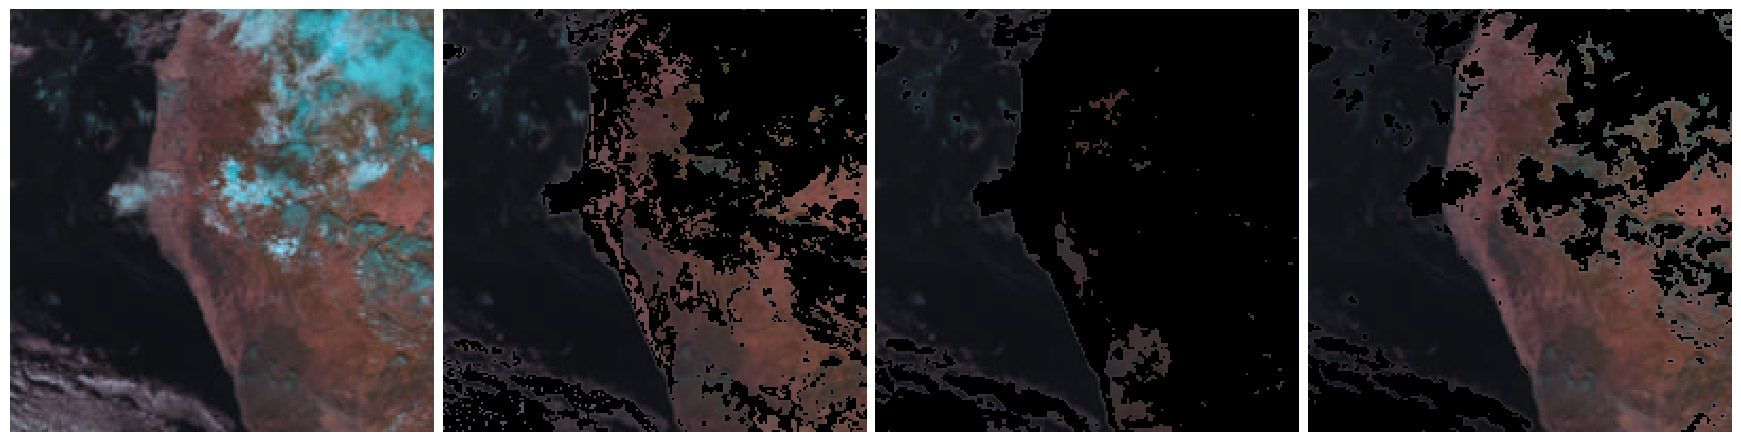
\includegraphics[width=1\textwidth]{compare_removal.png}
    \caption{Comparison of cloud removal algorithms on image from 2019-01-05 12:27:43.
    \\From left to right: original RGB image, thresholded image with values determined via inspection, thresholded image with single Otsu threshold value, and thresholded image using Otsu threshold values determined via use of masks over sea and land}
    \label{fig:iterav}
\end{figure}

Fig.~\ref{fig:iterav} illustrates the implementation of the different cloud removal methods we used to reduce pixel cloud noise, and shows their relative effectiveness. The three images on the far right of the figure are all RGB images in which a different thresholded mask was applied to each one. From left to right the masks were calcualted using threshold values determined by inspection, Otsu's algorithm, and the combination of Otsu's algorithm and a landmask. The separability measure of the global Otsu algorithm, the image second from the right, was calculated using Eq.~\ref{eq:sepm} and found to be $\eta = 0.932$.

\begin{figure}[h]
    \centering
    \includegraphics[width=1\textwidth]{g_Otsu_sealand_fail.png}
    \caption{Implementation of Otsu's algorithm. From left to right: Original greyscale image calculated from the square root of the mean sum squared of each channel (IR 1.6, VIS0.6, and VIS 0.8), histogram of distribution of pixel intensity values with red vertical line indicating the Otsu threshold value calculated, and thresholded mask determined from Otsu's algorithm}
    \label{fig:g_Otsu_fail}
\end{figure}

Fig.~\ref{fig:g_Otsu_fail} is a plot that illustrates the ineffectiveness of using a global Otsu threshold for a surface selection that straddles both land and sea pixels. The histogram in the figure, between the two images, shows the frequency of occurrence of different pixel values and where the optimum threshold value was calculated to lie. Two main peaks can be observed and it is these peaks that the algorithm identifies as foreground and background pixel values. Unfortunately, though the left hand peak does correspond to the darker pixels of the sea, the second peak is indicative of the land pixel values rather than those of clouds. Therefore by splitting these two peaks up the land pixels are grouped with the cloud pixels instead of the sea as is shown in the right hand thresholded image.

\begin{figure}
    \centering
    \includegraphics[width=1\textwidth]{landmask_Otsu_threshold_2019-01-05 122743.png}
    \caption{Implementation of Otsu's algorithm over the land using a landmask. From left to right: Original greyscale image of VIS 0.6 channel, histogram of distribution of pixel intensity values with red vertical line indicating the Otsu threshold value calculated, and thresholded mask over land determined from Otsu's algorithm}
    \label{fig:bOtsu_land}
\end{figure}

Fig.~\ref{fig:bOtsu_land}

\begin{figure}
    \centering
    \includegraphics[width=1\textwidth]{seamask_Otsu_threshold_2019-01-05 122743.png}
    \caption{Implementation of Otsu's algorithm over the sea using a reversed landmask. From left to right: Original greyscale image of VIS 0.8 channel, histogram of distribution of pixel intensity values with red vertical line indicating the Otsu threshold value calculated, and thresholded mask over sea determined from Otsu's algorithm}
    \label{fig:bOtsu_sea}
\end{figure}

Fig.~\ref{fig:bOtsu_sea}

\begin{figure}
    \centering
    \includegraphics[width=0.5\textwidth]{Otsu_av_mon.png}
    \caption{Averaged RGB image for January 2019 after the removal of cloud cover using land masks and Otsu's algorithm for optimum threshold identification}
    \label{fig:av_Otsu}
\end{figure}

Fig.~\ref{fig:av_Otsu} shows the cloud free averaged image of all the pixel values for the month of January 2019 via use of our masked Otsu's algorithm

\begin{figure}[h]
    \centering
    \includegraphics[width=0.5\textwidth]{Otsu_filled_2019-01-05 122743.png}
    \caption{New cloud free image for 2019-01-05 12:27:43, where cloudy pixels have been replaced by the corresponding pixels in the averaged January cloud free image}
    \label{fig:Otsu_fill}
\end{figure}

\begin{figure}[h]
    \centering
    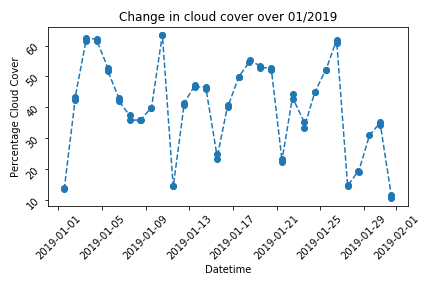
\includegraphics[totalheight=0.3\textheight]{cloud_percent_jan_southsea.png}
    \caption{Caption}
    \label{fig:cloud_pc_jan}
\end{figure}


\begin{figure}[h]
    \centering
    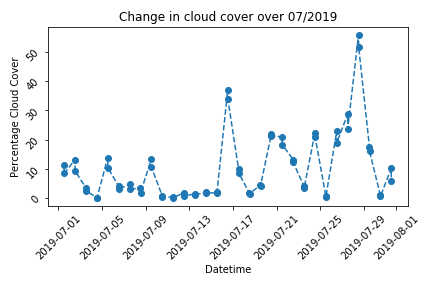
\includegraphics[totalheight=0.3\textheight]{cloud_percent_jul_southsea.png}
    \caption{Caption}
    \label{fig:cloud_pc_jul}
\end{figure}

\begin{figure}[h]
    \centering
    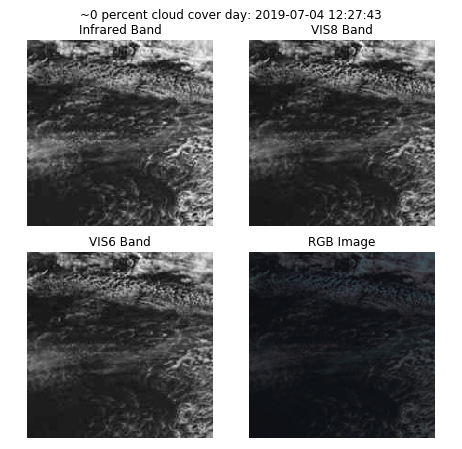
\includegraphics[totalheight=0.4\textheight]{0_per_day_sea.png}
    \caption{Caption}
    \label{fig:my_label}
\end{figure}


\begin{figure}[h]
    \centering
    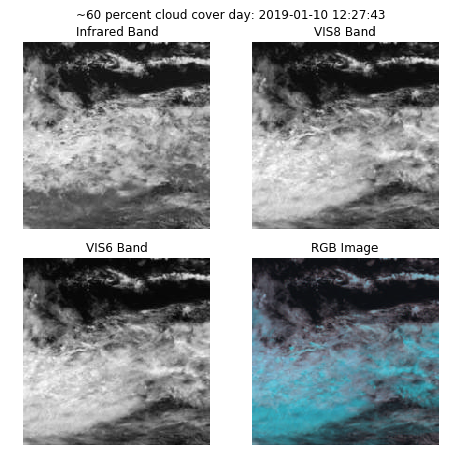
\includegraphics[totalheight=0.4\textheight]{60_per_day_sea.png}
    \caption{Caption}
    \label{fig:my_label}
\end{figure}


\begin{figure}[h]
    \centering
    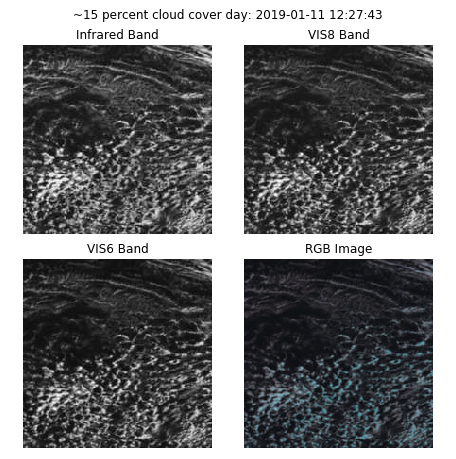
\includegraphics[totalheight=0.4\textheight]{15_per_day_sea_outlier.png}
    \caption{Caption}
    \label{fig:my_label}
\end{figure}


